\documentclass[12pt]{article}
\usepackage[utf8]{inputenc}
\usepackage{amsmath, amssymb}
\usepackage{xcolor}
\usepackage{geometry}
\usepackage{hyperref}
\usepackage{fancyhdr}
\usepackage{enumitem}
\usepackage{minted} % Code highlighting
\usepackage{booktabs} % Clean tables}
\usepackage{tikz}
\usetikzlibrary{shapes, arrows, positioning}

\geometry{margin=1in}
\hypersetup{colorlinks=true, linkcolor=blue, urlcolor=cyan}

\pagestyle{fancy}
\fancyhf{}
\fancyhead[L]{\textbf{\TOPICTITLE}}
\fancyhead[R]{\thepage}

% -------------------------------
% Topic Metadata
% -------------------------------
\newcommand{\TOPICTITLE}{Multiplexing and Demultiplexing}
\title{\TOPICTITLE\\\large Study-Ready Notes}
\author{Compiled by Andrew Photinakis}
\date{\today}

\setlength{\headheight}{15pt}

\begin{document}
\maketitle
\tableofcontents
\newpage

% This LaTeX file should be saved at: computer_networks/transport_layer/multiplexing_demultiplexing.tex

\section{Introduction to Multiplexing and Demultiplexing}

\begin{itemize}
    \item Part of transport-layer services in the protocol stack
    \item Essential for managing multiple simultaneous network connections
    \item Works alongside other transport layer functions:
          \begin{itemize}
              \item Connectionless transport: UDP
              \item Principles of reliable data transfer
              \item Connection-oriented transport: TCP
              \item Principles of congestion control
              \item TCP congestion control
              \item Evolution of transport-layer functionality
          \end{itemize}
\end{itemize}

\textcolor{blue}{[Summary: Multiplexing and demultiplexing are fundamental transport layer services that enable multiple applications to share network connections by properly directing data to the correct processes.]}

\section{Basic Concepts}

\subsection{Definitions}
\begin{itemize}
    \item \textbf{Multiplexing at sender}: Handling data from multiple sockets and adding transport header for later demultiplexing
    \item \textbf{Demultiplexing at receiver}: Using header information to deliver received segments to the correct socket
\end{itemize}

\begin{figure}[h]
    \centering
    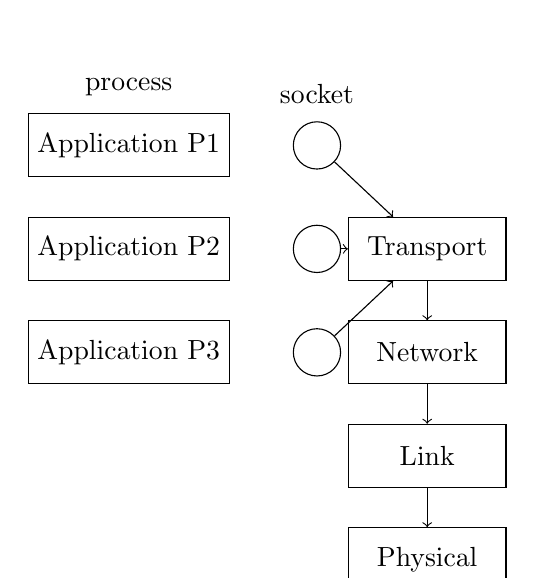
\begin{tikzpicture}[
            node distance=1.5cm,
            proc/.style={rectangle, draw, minimum width=2cm, minimum height=0.8cm},
            socket/.style={circle, draw, minimum size=0.6cm}
        ]
        % Sender side
        \node[proc] (app1) {Application P1};
        \node[proc, below=0.5cm of app1] (app2) {Application P2};
        \node[proc, below=0.5cm of app2] (app3) {Application P3};

        \node[socket, right=0.8cm of app1] (sock1) {};
        \node[socket, right=0.8cm of app2] (sock2) {};
        \node[socket, right=0.8cm of app3] (sock3) {};

        \node[proc, right=1.5cm of app2] (transport) {Transport};
        \node[proc, below=0.5cm of transport] (network) {Network};
        \node[proc, below=0.5cm of network] (link) {Link};
        \node[proc, below=0.5cm of link] (physical) {Physical};

        % Connections
        \draw[->] (sock1) -- (transport);
        \draw[->] (sock2) -- (transport);
        \draw[->] (sock3) -- (transport);
        \draw[->] (transport) -- (network);
        \draw[->] (network) -- (link);
        \draw[->] (link) -- (physical);

        % Labels
        \node[above=0.1cm of sock1] {socket};
        \node[above=0.1cm of app1] {process};

    \end{tikzpicture}
    \caption{Multiplexing: Multiple application processes sending data through sockets to transport layer}
    \label{fig:multiplexing_basic}
\end{figure}

\textcolor{orange}{[Mnemonic: "Mix Up, Sort Out" - Multiplexing mixes data from multiple sources, demultiplexing sorts it out to the right destinations.]}

\section{How Demultiplexing Works}

\subsection{Key Components}
\begin{itemize}
    \item Host receives IP datagrams with:
          \begin{itemize}
              \item Source IP address and destination IP address
              \item Each datagram carries one transport-layer segment
              \item Each segment has source and destination port numbers
          \end{itemize}
    \item Host uses \textbf{IP addresses and port numbers} to direct segments to appropriate sockets
\end{itemize}

\subsection{Transport Segment Format}
\begin{figure}[h]
    \centering
    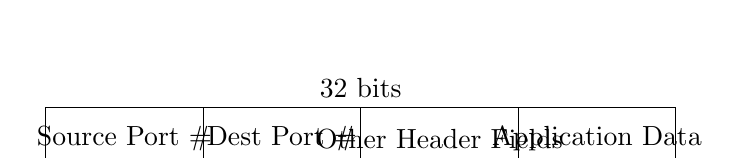
\begin{tikzpicture}
        \draw (0,0) rectangle (8,0.8);
        \draw (0,0) rectangle (2,0.8);
        \draw (2,0) rectangle (4,0.8);
        \draw (4,0) rectangle (6,0.8);
        \draw (6,0) rectangle (8,0.8);

        \node at (1,0.4) {Source Port \#};
        \node at (3,0.4) {Dest Port \#};
        \node at (5,0.4) {Other Header Fields};
        \node at (7,0.4) {Application Data};

        \node[above] at (4,0.8) {32 bits};
    \end{tikzpicture}
    \caption{TCP/UDP segment format showing key fields for demultiplexing}
    \label{fig:segment_format}
\end{figure}

\textcolor{blue}{[Summary: Demultiplexing uses IP addresses and port numbers from segment headers to route incoming data to the correct application socket, ensuring each process receives its intended data.]}

\section{Connectionless Demultiplexing (UDP)}

\subsection{Socket Creation and Configuration}
\begin{itemize}
    \item When creating UDP socket, must specify \textit{host-local} port number:
          \begin{minted}{java}
DatagramSocket mySocket1 = new DatagramSocket(12534);
    \end{minted}
    \item When creating datagram to send, must specify:
          \begin{itemize}
              \item Destination IP address
              \item Destination port number
          \end{itemize}
\end{itemize}

\subsection{Demultiplexing Process}
\begin{itemize}
    \item Receiving host checks destination port number in UDP segment
    \item Directs UDP segment to socket with that port number
    \item \textbf{Important}: IP/UDP datagrams with same destination port number but different source IP addresses and/or source port numbers are directed to the same socket
\end{itemize}

\begin{figure}[h]
    \centering
    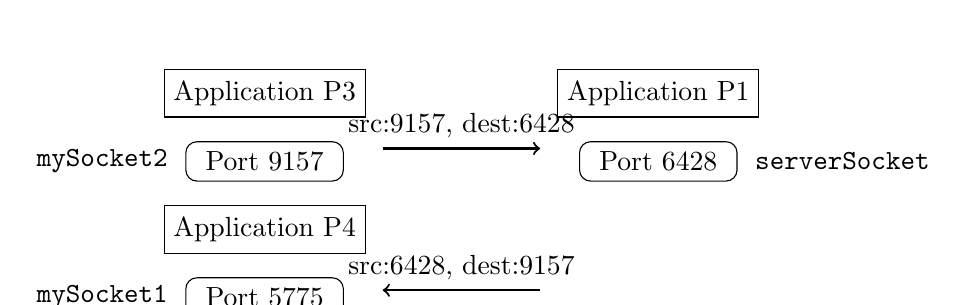
\begin{tikzpicture}[
            node distance=1cm,
            proc/.style={rectangle, draw, minimum width=2.5cm, minimum height=0.6cm},
            socket/.style={rectangle, draw, rounded corners, minimum width=2cm, minimum height=0.5cm}
        ]
        % Left side - applications
        \node[proc] (p3) at (0,0) {Application P3};
        \node[socket, below=0.3cm of p3] (sock2) {Port 9157};
        \node[proc, below=0.3cm of sock2] (p4) {Application P4};
        \node[socket, below=0.3cm of p4] (sock1) {Port 5775};

        % Right side - server
        \node[proc] (p1) at (5,0) {Application P1};
        \node[socket, below=0.3cm of p1] (server) {Port 6428};

        % Data flows
        \draw[->, thick] (1.5,-0.7) -- (3.5,-0.7) node[midway,above] {src:9157, dest:6428};
        \draw[->, thick] (3.5,-2.5) -- (1.5,-2.5) node[midway,above] {src:6428, dest:9157};

        % Labels
        \node[left=0.1cm of sock1] {\texttt{mySocket1}};
        \node[left=0.1cm of sock2] {\texttt{mySocket2}};
        \node[right=0.1cm of server] {\texttt{serverSocket}};

    \end{tikzpicture}
    \caption{Connectionless demultiplexing example showing UDP socket communication}
    \label{fig:udp_demux}
\end{figure}

\section{Connection-Oriented Demultiplexing (TCP)}

\subsection{TCP Socket Identification}
\begin{itemize}
    \item TCP socket identified by 4-tuple:
          \begin{itemize}
              \item Source IP address
              \item Source port number
              \item Destination IP address
              \item Destination port number
          \end{itemize}
    \item Demultiplexing uses \textbf{all four values} to direct segment to appropriate socket
\end{itemize}

\subsection{Server Socket Management}
\begin{itemize}
    \item Server may support many simultaneous TCP sockets
    \item Each socket identified by its own 4-tuple
    \item Each socket associated with a different connecting client
\end{itemize}

\begin{figure}[h]
    \centering
    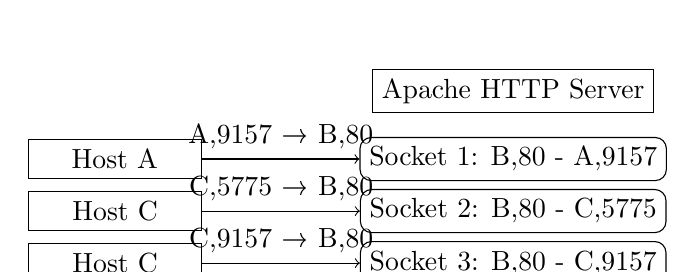
\begin{tikzpicture}[
            node distance=0.8cm,
            proc/.style={rectangle, draw, minimum width=2.2cm, minimum height=0.5cm},
            socket/.style={rectangle, draw, rounded corners, minimum width=2.5cm, minimum height=0.4cm}
        ]
        % Server
        \node[proc] (server) {Apache HTTP Server};
        \node[socket, below=0.3cm of server] (sock1) {Socket 1: B,80 - A,9157};
        \node[socket, below=0.1cm of sock1] (sock2) {Socket 2: B,80 - C,5775};
        \node[socket, below=0.1cm of sock2] (sock3) {Socket 3: B,80 - C,9157};

        % Clients
        \node[proc, left=2cm of sock1] (clientA) {Host A};
        \node[proc, left=2cm of sock2] (clientC1) {Host C};
        \node[proc, left=2cm of sock3] (clientC2) {Host C};

        % Connections
        \draw[->] (clientA.east) -- (sock1.west) node[midway,above] {A,9157 → B,80};
        \draw[->] (clientC1.east) -- (sock2.west) node[midway,above] {C,5775 → B,80};
        \draw[->] (clientC2.east) -- (sock3.west) node[midway,above] {C,9157 → B,80};

    \end{tikzpicture}
    \caption{Connection-oriented demultiplexing: Three segments with same destination (B,80) but different sources are directed to different sockets}
    \label{fig:tcp_demux}
\end{figure}

\textcolor{teal}{[Concept Map: Demultiplexing → UDP (destination port only) vs TCP (4-tuple: src/dest IP+port) → Enables multiple simultaneous connections → Essential for web servers handling multiple clients.]}

\section{Real-World Analogies}

\subsection{Airport Security Checkpoint}
\begin{itemize}
    \item \textbf{Multiplexing}: Multiple passengers from different flights going through same security checkpoint
    \item \textbf{Demultiplexing}: Passengers directed to correct gates based on flight information
    \item TSA Pre vs Main Checkpoint: Different processing based on passenger type
\end{itemize}

\subsection{Airline Boarding}
\begin{itemize}
    \item \textbf{Multiplexing}: All passengers for different flights in same terminal
    \item \textbf{Demultiplexing}: Passengers directed to specific gates (B14, 201E) based on destination
    \item Priority vs Economy: Different boarding groups within same flight
\end{itemize}

\subsection{Highway System}
\begin{itemize}
    \item \textbf{Multiplexing}: Multiple routes converging into main highways
    \item \textbf{Demultiplexing}: Exits directing traffic to specific destinations (14th St Downtown, Broadway)
\end{itemize}

\begin{table}[h]
    \centering
    \begin{tabular}{p{0.3\textwidth}p{0.3\textwidth}p{0.3\textwidth}}
        \toprule
        \textbf{Analogy} & \textbf{Multiplexing}                  & \textbf{Demultiplexing}                   \\
        \midrule
        Airport Security & All passengers through same checkpoint & Directed to correct gates based on flight \\
        Highway System   & Multiple routes merge into highway     & Exits direct to specific streets          \\
        Postal System    & All mail collected in same mailbox     & Sorted by address for delivery            \\
        \bottomrule
    \end{tabular}
    \caption{Real-world analogies for multiplexing and demultiplexing}
    \label{tab:analogies}
\end{table}

\section{Key Differences: UDP vs TCP Demultiplexing}

\begin{table}[h]
    \centering
    \begin{tabular}{p{0.45\textwidth}p{0.45\textwidth}}
        \toprule
        \textbf{Connectionless (UDP)}                    & \textbf{Connection-Oriented (TCP)}           \\
        \midrule
        Uses only destination port number                & Uses 4-tuple: source/destination IP and port \\
        Same socket receives all datagrams for that port & Separate socket for each connection          \\
        No connection establishment required             & Connection setup before data transfer        \\
        Stateless demultiplexing                         & Stateful demultiplexing                      \\
        Suitable for broadcast/multicast                 & Point-to-point communication                 \\
        \textbf{Example}: DNS queries                    & \textbf{Example}: HTTP web traffic           \\
        \bottomrule
    \end{tabular}
    \caption{Comparison of UDP vs TCP demultiplexing approaches}
    \label{tab:udp_vs_tcp_demux}
\end{table}

\textcolor{blue}{[Summary: UDP uses simple destination port-based demultiplexing where all traffic for a port goes to one socket, while TCP uses 4-tuple identification creating separate sockets for each connection, enabling multiple simultaneous conversations.]}

\section{Study Aids and Exam Preparation}

\subsection{Key Concepts to Master}
\begin{itemize}
    \item Understand the difference between multiplexing and demultiplexing
    \item Memorize the segment format and which fields are used for demultiplexing
    \item Know the exact 4-tuple used for TCP socket identification
    \item Be able to explain why TCP needs more complex demultiplexing than UDP
    \item Understand real-world analogies and how they relate to network concepts
\end{itemize}

\subsection{Practice Questions}
\begin{enumerate}
    \item \textbf{Compare and contrast} connectionless (UDP) and connection-oriented (TCP) demultiplexing. Why does TCP require a 4-tuple while UDP only needs destination port?

    \item Describe the process that occurs when a host receives a UDP datagram. How does it determine which socket should receive the data?

    \item A web server is running on port 80 and has three simultaneous TCP connections from different clients. Explain how the server keeps these connections separate and directs incoming segments to the correct socket.

    \item Using the \textbf{airport analogy}, explain how multiplexing and demultiplexing work in a network context. What represents ports? What represents sockets?

    \item What would happen if two different applications on the same host tried to bind to the same UDP port? What about the same TCP 4-tuple?
\end{enumerate}

\textcolor{orange}{[Mnemonic: "UDP: Simple Port, TCP: Four Report" - UDP uses simple port numbers, TCP requires four pieces of information (the 4-tuple).]}

\section{Summary}

\begin{itemize}
    \item Multiplexing and demultiplexing are based on segment/datagram header field values
    \item \textbf{UDP}: Demultiplexing using destination port number only
    \item \textbf{TCP}: Demultiplexing using 4-tuple (source and destination IP addresses and port numbers)
    \item Multiplexing/demultiplexing happen at all layers of the network stack
    \item These mechanisms enable multiple applications to share network resources efficiently
\end{itemize}

\section{References}
\begin{itemize}
    \item Kurose, J.F., \& Ross, K.W. (2020). \textit{Computer Networking: A Top-Down Approach (8th ed.)}. Pearson.
    \item Course: COMPSCI 453 Computer Networks, University of Massachusetts
    \item Professor: Jim Kurose, College of Information and Computer Sciences
    \item Textbook website: http://gala.cs.umass.edu/kurose\_ross
\end{itemize}

\end{document}